%                                                                 aa.dem
% AA vers. 8.2, LaTeX class for Astronomy & Astrophysics
% demonstration file
%                                                       (c) EDP Sciences
%-----------------------------------------------------------------------
%
%\documentclass[referee]{aa} % for a referee version
%\documentclass[onecolumn]{aa} % for a paper on 1 column  
%\documentclass[longauth]{aa} % for the long lists of affiliations 
%\documentclass[rnote]{aa} % for the research notes
%\documentclass[letter]{aa} % for the letters 
%\documentclass[bibyear]{aa} % if the references are not structured 
% according to the author-year natbib style

%
\documentclass{aa}  

%
\usepackage{graphicx}
%%%%%%%%%%%%%%%%%%%%%%%%%%%%%%%%%%%%%%%%
\usepackage{txfonts}
%%%%%%%%%%%%%%%%%%%%%%%%%%%%%%%%%%%%%%%%
%\usepackage[options]{hyperref}
% To add links in your PDF file, use the package "hyperref"
% with options according to your LaTeX or PDFLaTeX drivers.
%
\begin{document} 


   \title{Conceptual Designs of Photonic Propulsion Systems}

   %\subtitle{I. Overviewing the Lunar Propulsion Designs}

   \author{P. Nam
          \inst{1}
          \and
          V. Suri\inst{1}
          \and
          M. Welch\inst{1}
          \and
          C. Pennypacker\inst{1} [Order of Authors will be rearranged]
          }

   \institute{Lawrence Berkeley National Lab, University of California,
              1 Cyclotron Rd, Berkeley, CA 94720\\
              \email{crpennypacker@lbl.gov}
             }

% \abstract{}{}{}{}{} 
% 5 {} token are mandatory
 
  \abstract
  % context heading (optional)
  % {} leave it empty if necessary  
   {To investigate and build a conceptual design of the Lunar Photonic Propulsion System. The goal here is to make interplanetary travel possible by first setting a ideal location and making an effective design for the lunar system. This paper goes over the possible challenges that may arise in completing the project.}
  % aims heading (mandatory)
   {To transport payload and humans to Mars using a photonic propulsion system. The goal is to successfully land on Mars in around a month.}

   {}

   \keywords{photonic sails --
                the Moon --
                solar panels --
                Mars
               }

   \maketitle
%
%________________________________________________________________

\section{Introduction}

	The fastest manned spacecraft traveled at a maximum speed of 24,790 mph. When Mars and the Earth are at its closest, the probe can reach Mars in around 39 days. However, this phenomenon is the best case scenario and as such, rarely happens. The average distance from Earth to Mars is around 225 million km. When using the average distance and the velocity listed above, the time it takes to reach Mars increases to around 161 days. Both scenarios assume that the distance that the probe has to travel remains the same but in reality, this does not happen since planets travel in orbits around the Sun.
    
   The presence of humans will also limit how fast a rocket can go, since it limits how fast it can accelerate. Too high of an acceleration for a sustained amount of time can lead to loss of consciousness and even, death. For context, astronauts can experience 3-8 g's. Manned missions to Mars are in the works and decreasing the time that it takes to get to the planet would be ideal, both for mental and physical health reasons, as currently traveling to Mars may take up to 6-8 months.
    
    Photonic sails have the potential to be the answer to getting to Mars faster than any current rocket can with a low acceleration. Rocket propulsion is limited as the craft needs to carry its own fuel. With photonic propulsion, the spacecraft is not propelled by fuel. This type of propulsion requires a phased laser array that fires photons at a sail. The sail then reflects the photons, which imparts momentum onto the sail. 
    
    This paper will look into the advantages of a lunar photonics system propelling the \textit{Gadfly}, a hypothetical spacecraft that will determine the other parameters of the photonics system. The photonics system will consist of the laser array, the solar panels needed to power it, and the telescopes that will be used to lower the divergence of the laser.  It will also look into the challenges of building this system on the Moon and the ideal location to have it.
    
   
%__________________________________________________________________

\section{Advantages of a Lunar Photonics System}
%______________________________________________ 

%
	There is virtually no atmosphere on the Moon and as a result, it will be assumed to be a vacuum. The atmospheric turbulence on Earth leads to an increase in the divergence of lasers, but the Moon does not have this problem. Atmospheric turbulence can be mostly offset by adaptive optics but this only increases the number of components and cost of the overall system.
    
    This lack of an atmosphere also means that the Moon is more vulnerable to meteoroids. Space rocks smaller than 25 meters will likely burn up in the Earth's atmosphere, causing little or no damage but these rocks will impact the Moon. In addition to propelling The Gadfly, the laser array can be used to deflect and vaporize meteoroids that can cause serious damage to lunar infrastructure.
    
    The Moon has a slow rotation and revolution period (around 27 days for both), meaning the laser array can beam photons at the photonic sail for a longer, continuous amount of time. The Moon has around one-sixth of the Earth’s gravity, so the sails could start off closer to the surface compared to the Earth. This means that the laser accelerates the sails for a longer period of time before it diverges too much.
    
    The lack of an atmosphere and the weaker gravity means that it is much easier to launch the \textit{Gadfly} from the lunar surface. The laser array can only start firing once the \textit{Gadfly} is sufficiently elevated. This in turn reduces the amount of fuel required so that the sail can reach its target height.
   
    The Moon is also a great testing ground for the photonics system on Mars, due to its proximity to Earth and to the obstacles that it shares with Mars, in terms of constructing the system. This is relevant since Mars is chosen as the primary destination, meaning there needs to be a laser array on Mars to decelerate the craft. The two celestial bodies share a lack of protection against cosmic radiation, dust that can impede the structures in the system, and diminished sunlight availability. The solutions used to combat these issues on the Moon can be transferred over to Mars.

\section{The Gadfly}
\subsection{The Spacecraft}
	The Gadfly is a hypothetical spacecraft driven by photonic propulsion that will be used for this paper. Thrusters and a cockpit are added in the case of an emergency. Hypothermal stasis chambers are included so that the metabolism of the crew will go down by up to 95 percent. Since this spacecraft is carrying people, it needs to have a life support system as well and it will accelerate at a rate of .98m/$s^2$.Any part of the craft exposed to the photons will have the same reflective material so that no part of the ship absorbs the photons and becomes damaged by them. The craft will also have docking ports for rocket boosters that will help in the beginning and the end of its journey.
\subsection{The Solar Sails}
	The Gadfly will have a circular sail with a diameter of about 100 meters and the whole system, including four people, comes out to have a mass of 1000 kg. To simplify calculations, the sail will be assumed to have a reflectivity of 1. Current solar sails have thicknesses in the 1-10 µm range and are often made of aluminized polyimide. For a sail with a 100m diameter, it may be necessary to include graphene or carbon nanotubes as a base material to keep the sail intact. Since graphene is not a reflective material, it would need to be coated with a highly reflective material, like aluminized polyimide.
	
%______________________________________________________________
\section{The Flight Plan of The Gadfly}
\subsection{Ascent and Acceleration}
    The Gadfly will initially be launched into space by rockets. The laser array will align with the Gadfly as it elevates. Once The Gadfly is at a height where the gravitational force is less than the force that the photons exert on the sail, the rocket boosters will orient the craft so that when the sails deploy, it will face the laser array and not the craft. This maneuver is taken because if the craft is also hit by the photons, then it may negatively affect its motion. As previously stated, the craft will also have the same reflective material as a safety measure. This is in the event that the photons hit the craft, although if everything goes according to plan, all the photons should hit the sail. To preserve the reflective coating of the craft, it will only surround the craft when the lasers are firing. Once this happens, the rocket boosters will detach and fall safely back to the Moon to be reused. The boosters will also go back to the lunar surface in a path that does not impede with the lasers. Finally, the sails will then unfurl, along with the reflective coating, and the lasers will fire. 
\subsection{Deceleration and Descent}
    Once the Gadfly reaches the point where the laser array on Mars will start firing, the Gadfly will reorient itself so that the sails are pointed towards the Martian laser array. The lasers will continue firing until it reaches the point where rocket boosters will attach to the craft and help the craft descend onto the Martian surface. When the lasers stop firing, the sails and the reflective coating around the craft will fold up and then, it will be stored within the craft. 
 \begin{equation}
      a = \frac{GM}{r^{\mathrm{2}}}  \,,
   \end{equation}

\[
      \begin{array}{lp{0.8\linewidth}}
         M  & mass of the Moon     \\
         G               & gravitational constant                    \\
         r             & radius 
 \end{array}
   \]
\subsection{Height Calculations}
To find the height at which the gravitational acceleration equals the acceleration of the sail by photons(.98m/$s^2$), use the equation above. The gravitational acceleration at the surface of the Moon is 1.62m/$s^2$. The radius of the moon is 1,737km. The mass of the Moon and the gravitational constant remain constant, while the radius changes. The calculations of the equation above gives the answer of 1.286 times the radius of the Moon. This means that at around 497 km above the surface, the gravitational and the photonic acceleration will be equal. At a higher elevation than 497 km the lasers will be beamed to the sail. For the purposes of this paper, the lasers will be beamed at 550km, although the starting point is rather flexible. At this point, The Gadfly's acceleration will be low since it is not much higher than the gravitational acceleration. However, once it becomes significantly elevated (approximately four times the radius of the Moon), the acceleration of The Gadfly will essentially be .98/$s^2$.
\subsection{Divergence Calculation}
\[ 
      \begin{array}{lp{0.8\linewidth}}
         \theta  & laser divergence     \\
         D_{t}   & telescope diameter                   \\
         R_{s}   & sail radius			\\
         R_{li}  & initial laser radius \\
         R_{lf}  & final laser radius \\
         \lambda & wavelength of the laser \\
         d       & distance from the laser to the sail \\
         
         \end{array}
\]
 \begin{equation}
      \theta = \frac{\lambda}{D_{t}},  \\
 \end{equation}
 \begin{equation}
 	  p = \frac{h}{\lambda}   \\
 \end{equation}
  \begin{equation}
 	  R_{lf} = R_{li} + d\tan{\theta} \\
 \end{equation}
The wavelength of the laser is 10E-6m and the telescope diameter is 10 meters. At the starting point of 550km, the radius of the laser due to divergence will be 9.6E-4m. Using this series of equations, the distance at which the laser radius will diverge to the same radius as R_{s} is at 5E8m.


\subsection{Attitude Control}
After successfully launching and accelerating the Gadfly, the next step would be to be able to control the attitude of the craft. This can be achieved by embedding liquid crystal display(LCD) blocks that can control the reflectance of the solar sail, a method used and successfully tested by JAXA's solar sail IKAROS. Since this method uses photonic pressure to control attitude, extra propellant for this purpose would not be needed, meaning less fuel mass.
\section{Determining the Location of the Laser Array}
\begin{table}[h!]
      \caption[]{The orbital inclinations of the planets in the Solar System. }
         \label{KapSou}
     $$ 
         \begin{array}{p{0.5\linewidth}l}
            \hline
            \noalign{\smallskip}
            Planets     &  Orbital Inclination\\
            \noalign{\smallskip}
            \hline
            \noalign{\smallskip}
            Mercury     & 7^{\mathrm{o}}           \\
            Venus     & 3.39^{\mathrm{o}}           \\
            Earth &  0^{\mathrm{o}} (reference plane)     \\
%
          	\textbf{Mars}           & 1.85^{\mathrm{o}} \\
Jupiter     & 1.31^{\mathrm{o}}           \\     
Saturn     & 2.49^{\mathrm{o}}           \\
Uranus     & 0.77^{\mathrm{o}}           \\
Neptune    & 1.77^{\mathrm{o}}           \\
            \noalign{\smallskip}
            \hline
         \end{array}
     $$ 
   \end{table}
\subsection{The Lunar Equator}
Though the inclination of Mars is the most important number in Table 1, the orbital inclination data of the other planets are included to show the relatively coplanar nature of the Solar System.  Because of this coplanar nature, the lunar equator or near it is one of the best locations for a laser array, since an object pointed normal away from a level surface on the equator will be relatively close with the plane required to reach Mars. Thus, the lasers will not have to be facing close to the lunar surface to keep the Gadfly on the right trajectory to Mars. Pointing the lasers close to the surface can be potentially dangerous to anything near the array.

The lunar equator also experiences the most solar irradiance during the sunlit times since the surface and the rays are almost normal with each other. The lunar axial tilt is about 1.5 degrees, meaning that the rays will essentially be normal to the surface year round. This will be important for power generation via solar panels, which will be discussed later.
\subsection{Far Side of the Moon}
The far side of the Moon is also ideal, since it is always facing away from Earth due to tidal locking. The Earth will complicate any maneuvers to other celestial bodies as the photonic sails needs to avoid hitting the Earth and its atmosphere. The sail should have an unobstructed path to the desired location because an obstacle in the trajectory of the sail will either lead to more fuel being carried so that the craft can circumvent it or it limits when the sail can be launched.
\subsection{Flat Terrain}
The terrain for the array should be relatively flat. A level plane for all the laser in the array would simplify placement of the lasers. Unlike Earth, the Moon does not have an atmosphere that can burn up smaller meteorites, leading to more craters. Also, the Moon does not have natural processes like plate tectonic movement and erosion through water and wind to help level out the surface after an impact. The lunar environment makes it difficult to find flat surfaces but there are some locations that are relatively flat and fit all the other requirements listed above. There are three locations: the Hertzsprung, Korolev and Mendeleev crater, with diameters of 536, 423, and 325 km, respectively. The centers of all three craters listed above are between 6 and -6 degrees in latitude, and are located on the far side of the Moon. 
\subsection{Safety Considerations}
One of the main deterrents against a laser array on Earth or in its orbit for getting rid of space debris is because of its potential to damage satellites and other crafts in space. The locations mentioned also takes the potential weaponizing of the array into account and minimizes the impact that the lasers can have. The crater walls will protect anything outside of it from being hit by the lasers, if the lasers ever drastically veer off their intended positioning. The far side of the Moon would also be one of the best places to put a laser array, since the lasers will always be facing away from the Earth.
\begin{figure}[h!]
  \caption{A topographic map of the far side of the moon, with the equator drawn in and the craters labeled. A) Mendeleev B) Korolev C) Hertzsprung. The visible light colors make up the elevation, with red being the highest and dark blue/violet being the lowest.}
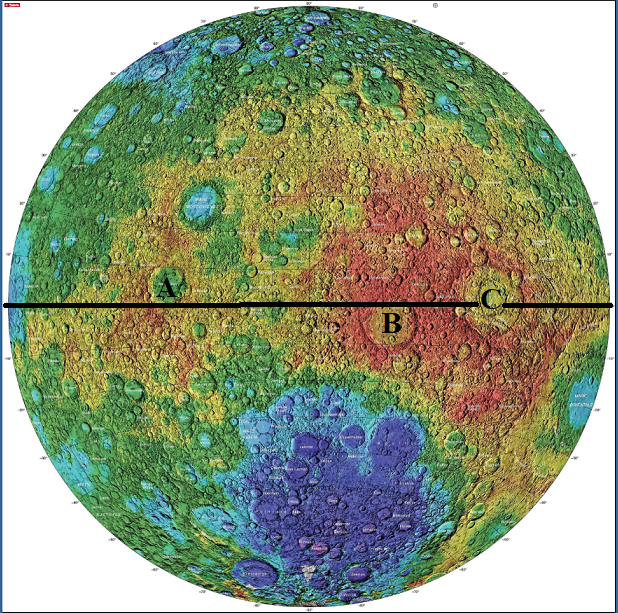
\includegraphics[width=0.48\textwidth]{Topographic_Map_of_the_Moon_s_Far_Side.png}
\end{figure}


%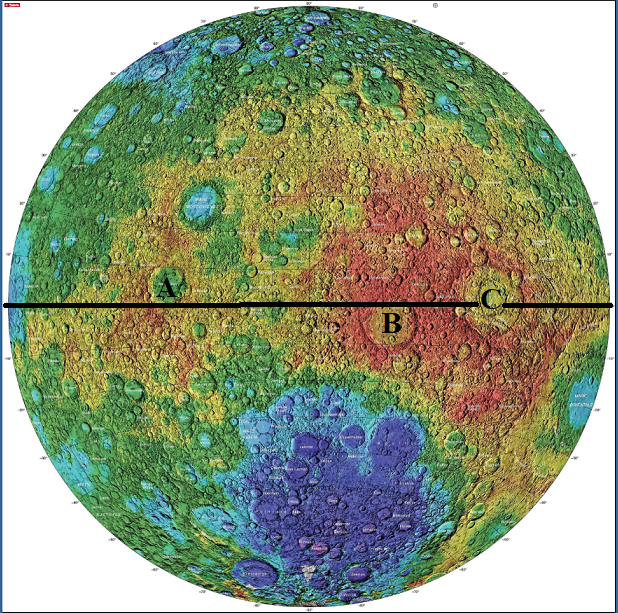
\includegraphics[width=0.5\textwidth]				{Topographic_Map_of_the_Moon_s_Far_Side.png}

%\captionof{Topographic_Map_of_the_Moon_s_Far_Side.png}{your caption text}


%______________________________________________________________
\section{Power Required}
\[
      \begin{array}{lp{0.8\linewidth}}
         p  & momentum of a photon     \\
         m  & mass of The Gadfly                    \\
         a  & acceleration of the gadfly				\\
         N_{p} & number of photons emitted per second  \\
         E  & energy of a photon \\
         P_{L}  & laser power \\
         h  & Planck's constant \\
         \lambda & wavelength of the laser \\
         c  & speed of light\\
         \end{array}
\]
 \begin{equation}
      E = \frac{\lambda c}{h},  \\
 \end{equation}
 \begin{equation}
 	  p = \frac{h}{\lambda}   \\
 \end{equation}
  \begin{equation}
 	  N_{p} = \frac{ma}{2p}   \\
 \end{equation}
 \begin{equation}
 	  P_{L} = N_{p}E\\
 \end{equation}

The wavelength of the laser and the mass and desired acceleration of The Gadfly have been mentioned previously. After inserting in the values into the equations, the amount of power from the lasers needed to accelerate The Gadfly to the desired amount comes out to be 147 GW. 
 
A report by Kulkarni and Lubin(2016) describes a laser array that is assumed to be 10km on a side and the laser power is assumed to be 70 GW. It also assumes that photons are not recycled, which this paper will also assume. Using the dimensions mentioned above and some scaling, the laser array will come out to be 220 $km^2$ , since around 147GW of laser power is needed to accelerate the Gadfly at a rate of .98 m/$s^2$. This means that the location for the laser array needs to be large enough, in terms of area, to hold this array. Each laser will have a power of 1 MW meaning 147,000 lasers are needed. However, this is a ridiculously high number of lasers and to make this system more feasible, the number almost certainly has to be reduced. 
\begin{table}[h!]
          \caption[]{The power level of each laser and the amount of lasers needed to meet 147 GW.}
         \label{KapSou}
     $$ 
         \begin{array}{p{0.5\linewidth}l}
            \hline
            \noalign{\smallskip}
            Laser Power     &  Number  of Lasers\\
            \noalign{\smallskip}
            \hline
            \noalign{\smallskip}
            1 MW   & 147,000           \\
            10 MW  & 14,700         \\
            100 MW & 1,470     \\
            1 GW   & 147                   \\
            \noalign{\smallskip}
            \hline
         \end{array}
     $$ 
   \end{table}
Increasing the power also increases the risk of destroying the sail. Though the reflectivity in this paper has been assumed to be 1 for all calculations, in reality, this number is not 1, although it can get very close. In his paper A Roadmap to Interstellar Flight, Lubin describes a solar sail design of 99.995\% reflectivity that uses metalized thin film plastic films with multi layer dielectric coatings can achieve very high reflectivity. Too strong of a laser can damage a sail, even if it's reflectivity is really close to 1. One possible solution is to increase the laser beam radius, to increase the area that the photons will hit. However, this will also result in an increase in wave interference between the lasers, which will result in less photons hitting the desired target. The right balance between laser power and beam radius will need to be found so that the sail and the amount of photons hitting it are not compromised.

\subsection{Laser Amplification}
However, building even a 750 KW laser outright is a practical impossibility. To create a higher power laser, power recycling mirrors are used to amplify the laser. The LIGO at Caltech uses these mirrors to amplify a 200 W beam up to 3750 times for a final resulting beam of 750KW. Assuming the same amplification, the amount of power needed to operate the laser will drastically decrease to 39.2 MW. 
\subsection{Reasons to Alter the Amount of Power Generated }
Note that the power required only takes into account the firing of the laser. More power is needed than the stated 39.2 MW to do the other actions such as actuating the motors that will move the lasers and change where it is pointing. Also, this calculation assumes a reflectivity of 1, meaning that more power would be needed to get an actual sail of the \textit{Gadfly's} mass to the desired acceleration.

Though the photons from the lasers will be the dominant factor in propelling the Gadfly, the Sun's photon will also play a role, increasing the amount of force that the craft experiences. However, to simplify calculations, none of these factors will be accounted for and 39.2 MW will be the number used when discussing the method of power generation.

\begin{figure}[h!]

 \caption{The average elemental composition of lunar regolith from the highlands and the mare}
 
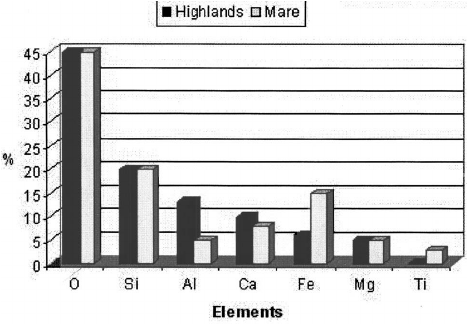
\includegraphics[width=0.48\textwidth]{Lunar Regolith Composition Graph.png}

\end{figure}

 \section{Method of Power Generation}
\subsection{Nuclear Power}
As mentioned previously, the lunar equator experiences a period of 14 days and 14 nights, meaning that solar power is only effective for half of a lunar period. However, nuclear power does not require sunlight, making it the ideal choice to power the laser array, not factoring cost. The required energy output is 39.2MW and the average nuclear power plant has an output of 1GW. According to a report by Schlissel and Biewald, however,  a 1,100 MW plant costs between \$6 billion and \$9 billion. The average nuclear power plant is many times greater in its power output than the power required for the lasers, meaning a relatively small nuclear power plant can be constructed. The cost of construction of this nuclear plant will be much higher on the Moon, since many materials will have to be transported to the Moon and the plant would have to be constructed there as well.
 \subsection{Solar Power}
Solar panels are a cheaper option since the cost to make solar panels is alleviated with the implementation of ISRU of the Moon's silicons to make the solar cells. According to Figure 2, silicon makes up around 20 percent of the lunar regolith, of which there is an abundance of on the Moon. The lunar regolith "is so plentiful, reaching depths of 4-5 meters (13-16.5 feet) in some places – and up to 15 meters (49 feet) in the older highland areas." 
	
    The lasers cannot be shot for half of the lunar period, using exclusively solar power. However, since the proposed region receives the highest amount of solar irradiance, less solar panels are needed, which means less cost. This decrease in cost outweigh the limitations of only being able to launch the photonic sails during the sunlit periods. Also, the panels can be stationary since the slight axial tilt on the Moon means that the panels will be close to or normal to the rays year round, if it's placed level relative to a flat surface.
\subsection{Solar Power and Energy Storage Hybrid}    
    However, this limited availability of sunlight can be alleviated with the introduction of an energy storage system, such as hydrogen fuel cells. The energy from the solar panels will not always be directed to the lasers, since the positioning of Mars and the Moon at times may make travel impossible. While the lasers are idle, the solar panels can be directed to an energy storage system. During the lunar night, the laser array can draw power from the storage system.
    
\section {Laser and Telescope Construction}
\subsection {Telescopes}
According to"To make a Hubble-sized moondust mirror(~8m), Chen calculates that astronauts would need to transport only 130 pounds (60 kg) of epoxy to the Moon along with 3 pounds (1.3 kg) of carbon nanotubes and less than 1 gram of aluminum. The bulk of the composite material—some 1,300 pounds (600 kilograms) of lunar dust—would be lying around on the Moon for free." Assuming that the telescope is going to be the same thickness as this hypothetical mirror and the only change is in the diameter, the materials needed after scaling to a 10 meter lens come out to be 203 lbs of epoxy, 4.68 lbs of carbon nanotubes, around 1 gram of aluminum, and 2,031 lbs of moondust. The epoxy and the carbon nanotubes will need to be transported from Earth but the bulk of the materials can be easily found on the Moon. 
\subsection {Lasers}
Lasers also require mirrors so these might also be made out of moon dust as well. They require a highly reflective lens and a partially reflective one. They also require a gain medium and a pump source but these components will most likely have to be made from materials transported from Earth. A protective shell is required to protect the inner components of the lasers from different lunar hazards. The photons exit from the partially reflective lens and these should only be exposed to the outside environment only during operation. The lasers will also need to be able to perform movements to change its elevation and its azimuthal angle. For any structural, load bearing components, aluminum alloys may be the best choice, with the explanation coming later in this paper.
\subsection {Laser Safety Measures}
Regardless of how much power each laser will have from Table 2, it will be strong enough to cause serious damage. Putting in a program that kills the laser if it veers drastically off course to an angle in which it is pointed near the surface is one measure that can be taken. Due to the low divergence of the laser, the reflected lasers can also pose a threat. There are two possible solutions to solve this. The first one is to create some program that can track where the lasers will be reflected and ensure that there is nothing in the path of the laser. The second one is to make a laser elevator. A laser elevator recycles the photons from a laser to increase the efficiency of photonic propulsion. It also provides a safe target for the reflected laser beams.

\section{Lunar Environment Hindrances to Construction and Possible Solutions}
The lasers, telescopes, and solar panels will all be exposed to the lunar environment. This results in all structures in this photonic system having some mechanism or method to deal with moonquakes, extreme temperature changes, slow heat rejection, solar flares and CMEs, galactic cosmic radiation(GCR), and lunar dust.

\subsection {Extreme Temperature Changes}
When sunlight hits the moon's surface, the temperature can reach 260 $^o$F (127 $^o$Celsius). When the sun goes down, temperatures can dip to -280 $^o$F (-173 $^o$C). Referring back to Figure 3, iron and aluminum are the most suitable elements, since they are relatively common in the lunar regolith. Out of these two elements, aluminum and its alloys are the most suited in handling the extreme temperature change. 

\subsection{Slow Heat Dissipation}
Since the Moon is essentially a vacuum, convection is eliminated and conduction would only occur with anything coming in contact with the lunar surface. As a result, losing heat would take longer on the Moon than on Earth. Certain measure may need to be taken for the solar panels, since they lose efficiency with increasing temperatures. The lasers will also need to have methods to dissipate heat more efficiently, since they will heat up during operation. Some possible solutions may be to include a radiator, thermoelectric cooler, and a white coating to reflect visible light.

Another possible method may be to minimize or maximize the amount of area that is in contact with the lunar surface. This would increase or decrease the amount of heat transfer via conduction. The depending factor would be the temperature of the lunar surface and the structure in question. More research would need to be done in this area if the amount of heat that these structures receive will jeopardize the whole operation. If the system can work without any measures taken, then that would be ideal in terms of total cost.
\subsection {Moonquakes}
Between 1972 and 1977, the Apollo seismic network saw twenty-eight of them; a few registered up to 5.5 on the Richter scale. Once they got going, all continued more than 10 minutes. Any habitat would have to be built of materials that are somewhat flexible. "A ductile structure's ability to contort and dissipate energy during an earthquake is advantageous as it will keep deforming without reaching ultimate failure or collapse." As previously mentioned, aluminum is ductile, which means it can better handle moonquakes. If more measures need to be taken, seismic dampers can also be added.  

\subsection {Micrometeorite Impacts}
"The actual risk to critical structures exposed on the
Moon is difficult to estimate, but the flux of meteoroids
represents a significant hazard and requires proper pro-
tection to critical structure—habitats, base support facilities, processing plants or research instruments, especially optical systems and detector packages—that are expected to last on the lunar surface for many years. Solar panels damaged by micrometeorites will need to be maintained and replaced gradually. The protective shell of the lasers and the exposing of the partially reflective mirror only during operation protect the components of the laser from micrometeorites.

\subsection {Solar Wind/Solar Flares/CMEs}
"Inside Earth's magnetosphere, strong electric currents can be generated by a CME strike," he explains. "Out in interplanetary space, however, the ambient magnetic field is much weaker and so those dangerous currents are missing."  In short, STEREO-A was in a good place to ride out the storm.
On July 2012, a powerful solar storm through Earth's orbit. Instead of hitting the Earth, the storm ended up hitting the STEREO-A spacecraft. However, the spacecraft survived because the magnetic field in interplanetary space is very weak. 

The Sun constantly releases solar wind, with varying degree. Intense outbursts of solar wind are called solar flares and CMEs, but most of these will not hit the Moon. However, when they do, electronics on the lunar surface may have an advantage as the Moon has no global magnetic field. The strongest magnetic field measurements recorded on the Moon only come about to on-hundredth of the strength of Earth's global field. This may allow them to ride out a solar flare/CME, like the STEREO-A spacecraft. A lack of a magnetic field protects electronics from a CME but it does not protect the system from galactic cosmic rays.

\subsection {Galactic Cosmic Rays}
Galactic cosmic rays(GCR) originate from sources outside of the Solar System. They are divided into two categories: primary and secondary cosmic rays. Earth's magnetic field and atmosphere shields the planet from 99.9 percent of the radiation from space. The Moon, however, does not have an atmosphere or a global magnetic field so these rays freely hit the lunar surface. In its revolution, the Moon does enter the Earth's magnetosphere for approximately 6 days. However, during the crossing, the moon comes in contact with a gigantic 'plasma sheet' of hot charged particles trapped in the tail.

One solution to this radiation problem is to use radiation resistant materials to protect any electronics susceptible to radiation damage. For energetic ion beams, a polyethylene(PE) target with its high hydrogen density is the most effective absorber of HZE particles for thick shields, while a polytetrafluoroethylene(PTFE) target with the heavier fluorine atoms appears to be more effective for thin shields, with respect to the production of secondary radiation. 

PTFE and PE cannot be made from the resources available on the Moon so this would have to be transported to the Moon. Another viable solution that would greatly reduce the need for these materials may be to have an underground site for components that are susceptible to damage by radiation and do not have to be on the surface. In addition to radiation protection, the regolith above this underground site would protect electronics from micrometeriod impacts, extreme temperature changes, and lunar dust, which will be discussed in the next section.
\subsection {Lunar Dust}
Lunar dust sticks onto surfaces very well due to it being abrasive from the lack of weathering and electrostatic from contact with the Sun's UV rays or plasma. So, the lasers need to be designed in a way so that lunar dust does not damage its inner components.  The dust can also impede any rotations and movements that the laser will need to make to accurately hit the sail. In addition, the accumulation of dust on solar panels will lower their efficiency.  To mitigate the effect of lunar dust, electrodynamic dust shield(EDS) devices may need to be installed. An experiment done by NASA in a vacuum chamber with simulated gravity found that 99 percent of the dust on surfaces protected by EDS devices were removed.

\section {Aluminum Alloys for Load Bearing Applications}
\subsection{Determining the Right Structural Material}
 Referring back to Figure 3, iron and aluminum are the most suitable elements, since they are relatively common in the lunar regolith and, when added with other elements that will have to be brought from Earth, become great materials for load bearing applications. However, after some analysis,   Out of these two elements, aluminum and its alloys are the most suited in handling the extreme temperature change.  For most aluminum alloys, strengths after significant times at temperatures above 150 to 200 $^o$C (300 to 400 $^o$F) are lower than those at room temperature, and the amount of the strength reduction may increase with both increasing temperature and/ or increasing time at an elevated temperature. The hottest that the lunar surface gets is below the elevated temperature range listed above. 
\subsection{Aluminum Alloys}
The changes in mechanical property for aluminum between cryogenic elevated temperatures are not so intensive compared to another materials such as steel and others. Aluminum alloys get stronger as the temperature decreases, even at minus 173 C.Alloys 5083 and 5456 have been tested in pressure vessels within the range from -195 to 65$^o$C. With these alloys, tensile strength increases 30 to 40\%, yield strength 5 to 10\% and elongation 60 to 100\% between room temperature and -195$^o$C. Higher tensile strength, yield strength, and elongation make aluminum alloys a better material in regards to bearing loads. Aluminum also keeps its ductility when exposed to cold temperature, whereas its iron alloy counterpart(steel), undergoes a transition when it gets sufficiently cold from a ductile to a brittle material. As stated previously, ductility plays a significant role in minimizing the impact that moonquakes would have on any structures.


\section{Conclusion}

	 Currently, transporting all the equipment from the Earth would be the only way to create a lunar photonics system but the cost of doing so would be prohibitive, at around 10,000 dollars a pound. This also does not count the cost of constructing the system and maintaining it once it is operational on the lunar surface. The current cost of transporting equipment combined with the sheer scale of the lasers, telescopes, and solar panels require a well-established and sophisticated lunar presence that utilizes ISRU to make this system anywhere remotely possible. A self-sufficient colony will also make maintenance and repair of the system less costly. However, humans have yet to create a permanent base on the Moon, though certain space agencies, such as the ESA, and private companies like Blue Origin, have expressed interest in establishing a permanent base in the next decade or two. If this comes to fruition in this time frame, the first step to a sophisticated lunar presence will happen in the near future.
     
     One of the first steps before building a laser array on the Moon is to build one on Earth, where construction and implementation of the whole system would be much easier and cheaper. Understanding how the laser array works on Earth will help in anticipating any problems that the potential lunar laser array may face. 
     
     This photonic system will also benefit greatly from advances in laser, telescope, reflective material, energy storage, and photovoltaic technology, which would decrease the cost of manufacturing the whole photonics system. To create this system, ISRU of the Moon will need to be heavily relied upon, since transporting material to the Moon will be very costly. However, certain parts of this system will inevitably need to be transported from Earth, meaning this system will benefit greatly from a reduction in the cost of transporting payload from the Earth to space. If this reduction is drastic enough, it may be possible to transport the whole system at a reasonable cost.
     
     Briefly mentioned, laser elevators, which recycle photons, can be very helpful and may be necessary due to the sheer amount of equipment required to move The Gadfly at the desired acceleration. It has the potential of increasing the efficiency of the system by a thousand, up to a certain distance known as the diffraction distance, beyond which the efficiency decreases.
   \begin{enumerate}
      \item The conditions for the stability of static, radiative
         layers in gas spheres, as described by Baker's (\cite{baker})
         standard one-zone model, can be expressed as stability
         equations of state. These stability equations of state depend
         only on the local thermodynamic state of the layer.
      \item If the constitutive relations -- equations of state and
         Rosseland mean opacities -- are specified, the stability
         equations of state can be evaluated without specifying
         properties of the layer.
      \item For solar composition gas the $\kappa$-mechanism is
         working in the regions of the ice and dust features
         in the opacities, the $\mathrm{H}_2$ dissociation and the
         combined H, first He ionization zone, as
         indicated by vibrational instability. These regions
         of instability are much larger in extent and degree of
         instability than the second He ionization zone
         that drives the Cephe{\"\i}d pulsations.
   \end{enumerate}

\begin{acknowledgements}
\end{acknowledgements}


%-------------------------------------------------------------------

\begin{thebibliography}{}

  
\end{thebibliography}

\end{document}

%%%%%%%%%%%%%%%%%%%%%%%%%%%%%%%%%%%%%%%%%%%%%%%%%%%%%%%%%%%%%%
Examples for figures using graphicx
A guide "Using Imported Graphics in LaTeX2e"  (Keith Reckdahl)
is available on a lot of LaTeX public servers or ctan mirrors.
The file is : epslatex.pdf 
%%%%%%%%%%%%%%%%%%%%%%%%%%%%%%%%%%%%%%%%%%%%%%%%%%%%%%%%%%%%%%

%_____________________________________________________________
%                 A figure as large as the width of the column
%-------------------------------------------------------------
   \begin{figure}
   \centering
   \includegraphics[width=\hsize]{empty.eps}
      \caption{Vibrational stability equation of state
               $S_{\mathrm{vib}}(\lg e, \lg \rho)$.
               $>0$ means vibrational stability.
              }
         \label{FigVibStab}
   \end{figure}
%
%_____________________________________________________________
%                                    One column rotated figure
%-------------------------------------------------------------
   \begin{figure}
   \centering
   \includegraphics[angle=-90,width=3cm]{empty.eps}
      \caption{Vibrational stability equation of state
               $S_{\mathrm{vib}}(\lg e, \lg \rho)$.
               $>0$ means vibrational stability.
              }
         \label{FigVibStab}
   \end{figure}
%
%_____________________________________________________________
%                        Figure with caption on the right side 
%-------------------------------------------------------------
   \begin{figure}
   \sidecaption
   \includegraphics[width=3cm]{empty.eps}
      \caption{Vibrational stability equation of state
               $S_{\mathrm{vib}}(\lg e, \lg \rho)$.
               $>0$ means vibrational stability.
              }
         \label{FigVibStab}
   \end{figure}
%
%_____________________________________________________________
%
%_____________________________________________________________
%                                Figure with a new BoundingBox 
%-------------------------------------------------------------
   \begin{figure}
   \centering
   \includegraphics[bb=10 20 100 300,width=3cm,clip]{empty.eps}
      \caption{Vibrational stability equation of state
               $S_{\mathrm{vib}}(\lg e, \lg \rho)$.
               $>0$ means vibrational stability.
              }
         \label{FigVibStab}
   \end{figure}
%
%_____________________________________________________________
%
%_____________________________________________________________
%                                      The "resizebox" command 
%-------------------------------------------------------------
   \begin{figure}
   \resizebox{\hsize}{!}
            {\includegraphics[bb=10 20 100 300,clip]{empty.eps}
      \caption{Vibrational stability equation of state
               $S_{\mathrm{vib}}(\lg e, \lg \rho)$.
               $>0$ means vibrational stability.
              }
         \label{FigVibStab}
   \end{figure}
%
%______________________________________________________________
%
%_____________________________________________________________
%                                             Two column Figure 
%-------------------------------------------------------------
   \begin{figure*}
   \resizebox{\hsize}{!}
            {\includegraphics[bb=10 20 100 300,clip]{empty.eps}
      \caption{Vibrational stability equation of state
               $S_{\mathrm{vib}}(\lg e, \lg \rho)$.
               $>0$ means vibrational stability.
              }
         \label{FigVibStab}
   \end{figure*}
%
%______________________________________________________________
%
%_____________________________________________________________
%                                             Simple A&A Table
%_____________________________________________________________
%
\begin{table}
\caption{Nonlinear Model Results}             % title of Table
\label{table:1}      % is used to refer this table in the text
\centering                          % used for centering table
\begin{tabular}{c c c c}        % centered columns (4 columns)
\hline\hline                 % inserts double horizontal lines
HJD & $E$ & Method\#2 & Method\#3 \\    % table heading 
\hline                        % inserts single horizontal line
   1 & 50 & $-837$ & 970 \\      % inserting body of the table
   2 & 47 & 877    & 230 \\
   3 & 31 & 25     & 415 \\
   4 & 35 & 144    & 2356 \\
   5 & 45 & 300    & 556 \\ 
\hline                                   %inserts single line
\end{tabular}
\end{table}
%
%_____________________________________________________________
%                                             Two column Table 
%_____________________________________________________________
%
\begin{table*}
\caption{Nonlinear Model Results}             
\label{table:1}      
\centering          
\begin{tabular}{c c c c l l l }     % 7 columns 
\hline\hline       
                      % To combine 4 columns into a single one 
HJD & $E$ & Method\#2 & \multicolumn{4}{c}{Method\#3}\\ 
\hline                    
   1 & 50 & $-837$ & 970 & 65 & 67 & 78\\  
   2 & 47 & 877    & 230 & 567& 55 & 78\\
   3 & 31 & 25     & 415 & 567& 55 & 78\\
   4 & 35 & 144    & 2356& 567& 55 & 78 \\
   5 & 45 & 300    & 556 & 567& 55 & 78\\
\hline                  
\end{tabular}
\end{table*}
%
%-------------------------------------------------------------
%                                          Table with notes 
%-------------------------------------------------------------
%
% A single note
\begin{table}
\caption{\label{t7}Spectral types and photometry for stars in the
  region.}
\centering
\begin{tabular}{lccc}
\hline\hline
Star&Spectral type&RA(J2000)&Dec(J2000)\\
\hline
69           &B1\,V     &09 15 54.046 & $-$50 00 26.67\\
49           &B0.7\,V   &*09 15 54.570& $-$50 00 03.90\\
LS~1267~(86) &O8\,V     &09 15 52.787&11.07\\
24.6         &7.58      &1.37 &0.20\\
\hline
LS~1262      &B0\,V     &09 15 05.17&11.17\\
MO 2-119     &B0.5\,V   &09 15 33.7 &11.74\\
LS~1269      &O8.5\,V   &09 15 56.60&10.85\\
\hline
\end{tabular}
\tablefoot{The top panel shows likely members of Pismis~11. The second
panel contains likely members of Alicante~5. The bottom panel
displays stars outside the clusters.}
\end{table}
%
% More notes
%
\begin{table}
\caption{\label{t7}Spectral types and photometry for stars in the
  region.}
\centering
\begin{tabular}{lccc}
\hline\hline
Star&Spectral type&RA(J2000)&Dec(J2000)\\
\hline
69           &B1\,V     &09 15 54.046 & $-$50 00 26.67\\
49           &B0.7\,V   &*09 15 54.570& $-$50 00 03.90\\
LS~1267~(86) &O8\,V     &09 15 52.787&11.07\tablefootmark{a}\\
24.6         &7.58\tablefootmark{1}&1.37\tablefootmark{a}   &0.20\tablefootmark{a}\\
\hline
LS~1262      &B0\,V     &09 15 05.17&11.17\tablefootmark{b}\\
MO 2-119     &B0.5\,V   &09 15 33.7 &11.74\tablefootmark{c}\\
LS~1269      &O8.5\,V   &09 15 56.60&10.85\tablefootmark{d}\\
\hline
\end{tabular}
\tablefoot{The top panel shows likely members of Pismis~11. The second
panel contains likely members of Alicante~5. The bottom panel
displays stars outside the clusters.\\
\tablefoottext{a}{Photometry for MF13, LS~1267 and HD~80077 from
Dupont et al.}
\tablefoottext{b}{Photometry for LS~1262, LS~1269 from
Durand et al.}
\tablefoottext{c}{Photometry for MO2-119 from
Mathieu et al.}
}
\end{table}
%
%-------------------------------------------------------------
%                                       Table with references 
%-------------------------------------------------------------
%
\begin{table*}[h]
 \caption[]{\label{nearbylistaa2}List of nearby SNe used in this work.}
\begin{tabular}{lccc}
 \hline \hline
  SN name &
  Epoch &
 Bands &
  References \\
 &
  (with respect to $B$ maximum) &
 &
 \\ \hline
1981B   & 0 & {\it UBV} & 1\\
1986G   &  $-$3, $-$1, 0, 1, 2 & {\it BV}  & 2\\
1989B   & $-$5, $-$1, 0, 3, 5 & {\it UBVRI}  & 3, 4\\
1990N   & 2, 7 & {\it UBVRI}  & 5\\
1991M   & 3 & {\it VRI}  & 6\\
\hline
\noalign{\smallskip}
\multicolumn{4}{c}{ SNe 91bg-like} \\
\noalign{\smallskip}
\hline
1991bg   & 1, 2 & {\it BVRI}  & 7\\
1999by   & $-$5, $-$4, $-$3, 3, 4, 5 & {\it UBVRI}  & 8\\
\hline
\noalign{\smallskip}
\multicolumn{4}{c}{ SNe 91T-like} \\
\noalign{\smallskip}
\hline
1991T   & $-$3, 0 & {\it UBVRI}  &  9, 10\\
2000cx  & $-$3, $-$2, 0, 1, 5 & {\it UBVRI}  & 11\\ %
\hline
\end{tabular}
\tablebib{(1)~\citet{branch83};
(2) \citet{phillips87}; (3) \citet{barbon90}; (4) \citet{wells94};
(5) \citet{mazzali93}; (6) \citet{gomez98}; (7) \citet{kirshner93};
(8) \citet{patat96}; (9) \citet{salvo01}; (10) \citet{branch03};
(11) \citet{jha99}.
}
\end{table}
%_____________________________________________________________
%                      A rotated Two column Table in landscape  
%-------------------------------------------------------------
\begin{sidewaystable*}
\caption{Summary for ISOCAM sources with mid-IR excess 
(YSO candidates).}\label{YSOtable}
\centering
\begin{tabular}{crrlcl} 
\hline\hline             
ISO-L1551 & $F_{6.7}$~[mJy] & $\alpha_{6.7-14.3}$ 
& YSO type$^{d}$ & Status & Comments\\
\hline
  \multicolumn{6}{c}{\it New YSO candidates}\\ % To combine 6 columns into a single one
\hline
  1 & 1.56 $\pm$ 0.47 & --    & Class II$^{c}$ & New & Mid\\
  2 & 0.79:           & 0.97: & Class II ?     & New & \\
  3 & 4.95 $\pm$ 0.68 & 3.18  & Class II / III & New & \\
  5 & 1.44 $\pm$ 0.33 & 1.88  & Class II       & New & \\
\hline
  \multicolumn{6}{c}{\it Previously known YSOs} \\
\hline
  61 & 0.89 $\pm$ 0.58 & 1.77 & Class I & \object{HH 30} & Circumstellar disk\\
  96 & 38.34 $\pm$ 0.71 & 37.5& Class II& MHO 5          & Spectral type\\
\hline
\end{tabular}
\end{sidewaystable*}
%_____________________________________________________________
%                      A rotated One column Table in landscape  
%-------------------------------------------------------------
\begin{sidewaystable}
\caption{Summary for ISOCAM sources with mid-IR excess 
(YSO candidates).}\label{YSOtable}
\centering
\begin{tabular}{crrlcl} 
\hline\hline             
ISO-L1551 & $F_{6.7}$~[mJy] & $\alpha_{6.7-14.3}$ 
& YSO type$^{d}$ & Status & Comments\\
\hline
  \multicolumn{6}{c}{\it New YSO candidates}\\ % To combine 6 columns into a single one
\hline
  1 & 1.56 $\pm$ 0.47 & --    & Class II$^{c}$ & New & Mid\\
  2 & 0.79:           & 0.97: & Class II ?     & New & \\
  3 & 4.95 $\pm$ 0.68 & 3.18  & Class II / III & New & \\
  5 & 1.44 $\pm$ 0.33 & 1.88  & Class II       & New & \\
\hline
  \multicolumn{6}{c}{\it Previously known YSOs} \\
\hline
  61 & 0.89 $\pm$ 0.58 & 1.77 & Class I & \object{HH 30} & Circumstellar disk\\
  96 & 38.34 $\pm$ 0.71 & 37.5& Class II& MHO 5          & Spectral type\\
\hline
\end{tabular}
\end{sidewaystable}
%
%_____________________________________________________________
%                              Table longer than a single page  
%-------------------------------------------------------------
% All long tables will be placed automatically at the end, after 
%                                        \end{thebibliography}
%
\begin{longtab}
\begin{longtable}{lllrrr}
\caption{\label{kstars} Sample stars with absolute magnitude}\\
\hline\hline
Catalogue& $M_{V}$ & Spectral & Distance & Mode & Count Rate \\
\hline
\endfirsthead
\caption{continued.}\\
\hline\hline
Catalogue& $M_{V}$ & Spectral & Distance & Mode & Count Rate \\
\hline
\endhead
\hline
\endfoot
%%
Gl 33    & 6.37 & K2 V & 7.46 & S & 0.043170\\
Gl 66AB  & 6.26 & K2 V & 8.15 & S & 0.260478\\
Gl 68    & 5.87 & K1 V & 7.47 & P & 0.026610\\
         &      &      &      & H & 0.008686\\
Gl 86 
\footnote{Source not included in the HRI catalog. See Sect.~5.4.2 for details.}
         & 5.92 & K0 V & 10.91& S & 0.058230\\
\end{longtable}
\end{longtab}
%
%_____________________________________________________________
%                              Table longer than a single page
%                                             and in landscape 
%  In the preamble, use:       \usepackage{lscape}
%-------------------------------------------------------------
% All long tables will be placed automatically at the end, after
%                                        \end{thebibliography}
%
\begin{longtab}
\begin{landscape}
\begin{longtable}{lllrrr}
\caption{\label{kstars} Sample stars with absolute magnitude}\\
\hline\hline
Catalogue& $M_{V}$ & Spectral & Distance & Mode & Count Rate \\
\hline
\endfirsthead
\caption{continued.}\\
\hline\hline
Catalogue& $M_{V}$ & Spectral & Distance & Mode & Count Rate \\
\hline
\endhead
\hline
\endfoot
%%
Gl 33    & 6.37 & K2 V & 7.46 & S & 0.043170\\
Gl 66AB  & 6.26 & K2 V & 8.15 & S & 0.260478\\
Gl 68    & 5.87 & K1 V & 7.47 & P & 0.026610\\
         &      &      &      & H & 0.008686\\
Gl 86
\footnote{Source not included in the HRI catalog. See Sect.~5.4.2 for details.}
         & 5.92 & K0 V & 10.91& S & 0.058230\\
\end{longtable}
\end{landscape}
\end{longtab}
%
% Online Material
%_____________________________________________________________
%        Online appendices have to be placed at the end, after
%                                        \end{thebibliography}
%-------------------------------------------------------------
\end{thebibliography}

\Online

\begin{appendix} %First online appendix
\section{Background galaxy number counts and shear noise-levels}
Because the optical images used in this analysis...

\begin{figure*}
\centering
\includegraphics[width=16.4cm,clip]{1787f24.ps}
\caption{Plotted above...}
\label{appfig}
\end{figure*}

Because the optical images...
\end{appendix}

\begin{appendix} %Second online appendix
These studies, however, have faced...
\end{appendix}

\end{document}
%
%_____________________________________________________________
%        Some tables or figures are in the printed version and
%                      some are only in the electronic version
%-------------------------------------------------------------
%
% Leave all the tables or figures in the text, at their right place 
% and use the commands \onlfig{} and \onltab{}. These elements
% will be automatically placed at the end, in the section
% Online material.

\documentclass{aa}
...
\begin{document}
text of the paper...
\begin{figure*}%f1
\includegraphics[width=10.9cm]{1787f01.eps}
\caption{Shown in greyscale is a...}
\label{cl12301}}
\end{figure*}
...
from the intrinsic ellipticity distribution.
% Figure 2 available electronically only
\onlfig{
\begin{figure*}%f2
\includegraphics[width=11.6cm]{1787f02.eps}
\caption {Shown in greyscale...}
\label{cl1018}
\end{figure*}
}

% Figure 3 available electronically only
\onlfig{
\begin{figure*}%f3
\includegraphics[width=11.2cm]{1787f03.eps}
\caption{Shown in panels...}
\label{cl1059}
\end{figure*}
}

\begin{figure*}%f4
\includegraphics[width=10.9cm]{1787f04.eps}
\caption{Shown in greyscale is...}
\label{cl1232}}
\end{figure*}

\begin{table}%t1
\caption{Complexes characterisation.}\label{starbursts}
\centering
\begin{tabular}{lccc}
\hline \hline
Complex & $F_{60}$ & 8.6 &  No. of  \\
...
\hline
\end{tabular}
\end{table}
The second method produces...

% Figure 5 available electronically only
\onlfig{
\begin{figure*}%f5
\includegraphics[width=11.2cm]{1787f05.eps}
\caption{Shown in panels...}
\label{cl1238}}
\end{figure*}
}

As can be seen, in general the deeper...
% Table 2 available electronically only
\onltab{
\begin{table*}%t2
\caption{List of the LMC stellar complexes...}\label{Properties}
\centering
\begin{tabular}{lccccccccc}
\hline  \hline
Stellar & RA & Dec & ...
...
\hline
\end{tabular}
\end{table*}
}

% Table 3 available electronically only
\onltab{
\begin{table*}%t3
\caption{List of the derived...}\label{IrasFluxes}
\centering
\begin{tabular}{lcccccccccc}
\hline \hline
Stellar & $f12$ & $L12$ &...
...
\hline
\end{tabular}
\end{table*}
}
%
%-------------------------------------------------------------
%     For the online material, table longer than a single page
%                 In the preamble for landscape case, use : 
%                                          \usepackage{lscape}
%-------------------------------------------------------------
\documentclass{aa}
\usepackage[varg]{txfonts}
\usepackage{graphicx}
\usepackage{lscape}

\begin{document}
text of the paper
% Table will be print automatically at the end, in the section Online material.
\onllongtab{
\begin{longtable}{lrcrrrrrrrrl}
\caption{Line data and abundances ...}\\
\hline
\hline
Def & mol & Ion & $\lambda$ & $\chi$ & $\log gf$ & N & e &  rad & $\delta$ & $\delta$ 
red & References \\
\hline
\endfirsthead
\caption{Continued.} \\
\hline
Def & mol & Ion & $\lambda$ & $\chi$ & $\log gf$ & B & C &  rad & $\delta$ & $\delta$ 
red & References \\
\hline
\endhead
\hline
\endfoot
\hline
\endlastfoot
A & CH & 1 &3638 & 0.002 & $-$2.551 &  &  &  & $-$150 & 150 &  Jorgensen et al. (1996) \\                    
\end{longtable}
}% End onllongtab

% Or for landscape, large table:

\onllongtab{
\begin{landscape}
\begin{longtable}{lrcrrrrrrrrl}
...
\end{longtable}
\end{landscape}
}% End onllongtab